\documentclass{report}
\usepackage{graphicx}
\usepackage[top=1in, bottom=1in, left=0.5in, right=0.5in]{geometry}
\usepackage{lscape}
\graphicspath{ {images/} }

\title{Amplifier Topologies}
\author{Simon Hobbs}
\newcommand{\imwidth}{0.2\textwidth}

\begin{document}
\maketitle

\chapter{Basic Single BJT}
\section{Common-Emitter}
\begin{figure}
\centering
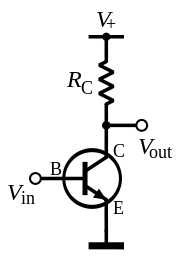
\includegraphics[width = \imwidth]{NPN_common_emitter}
\caption{}
\end{figure}

\section{Common-Base}
\begin{figure}
\centering
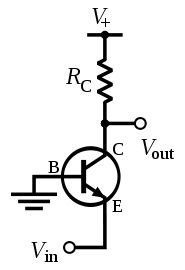
\includegraphics[width = \imwidth]{NPN_common_base}
\caption{}
\end{figure}

\section{Common-Collector}
AKA emitter follower
\begin{figure}
\centering
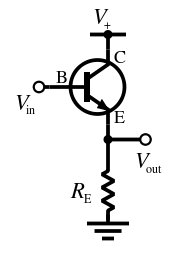
\includegraphics[width = \imwidth]{NPN_common_collector}
\caption{}
\end{figure}


\chapter{Basic Single FET}
\section{Common-Source}
\section{Common-Gate}
\section{Common-Drain}

\chapter{Multisection BJT Amps}
\section{Cascade}
\section{Cascode}

\begin{figure}
\centering
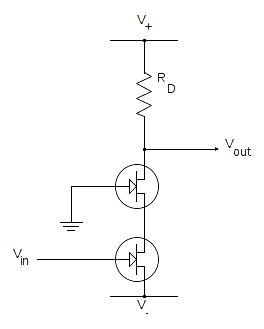
\includegraphics[width = \imwidth]{CascodeWithNegative}
\caption{}
\end{figure}


\section{Darlington}
\section{Differential Emitter-Coupled}
AKA Long-tail
\section{Current Mirrors}

\chapter{Amplifier Concepts}
\section{Emitter Degeneration}
\section{Bootstraping}


\end{document}
